%% A "teaser" image appears between the author and affiliation
%% information and the body of the document, and typically spans the
%% page.
\setlength{\resLen}{6.9in}
\begin{teaserfigure}
	\centering
	\addtolength{\tabcolsep}{-4pt}
	\begin{tabular}{cc}
		\raisebox{0.225in}{\rotatebox[origin=c]{90}{\small Input}} &
		
\includegraphics[width=\resLen]{teaser/refs.jpg}
		\\[-2pt]
		\raisebox{0.45in}{\rotatebox[origin=c]{90}{\small Rendering}} &
		\animategraphics[width=\resLen,loop,alttext=]{5}{teaser/teaser_}{001}{024}
		\\[-2pt]
		\raisebox{0.45in}{\rotatebox[origin=c]{90}{\small Estimated maps}} &
		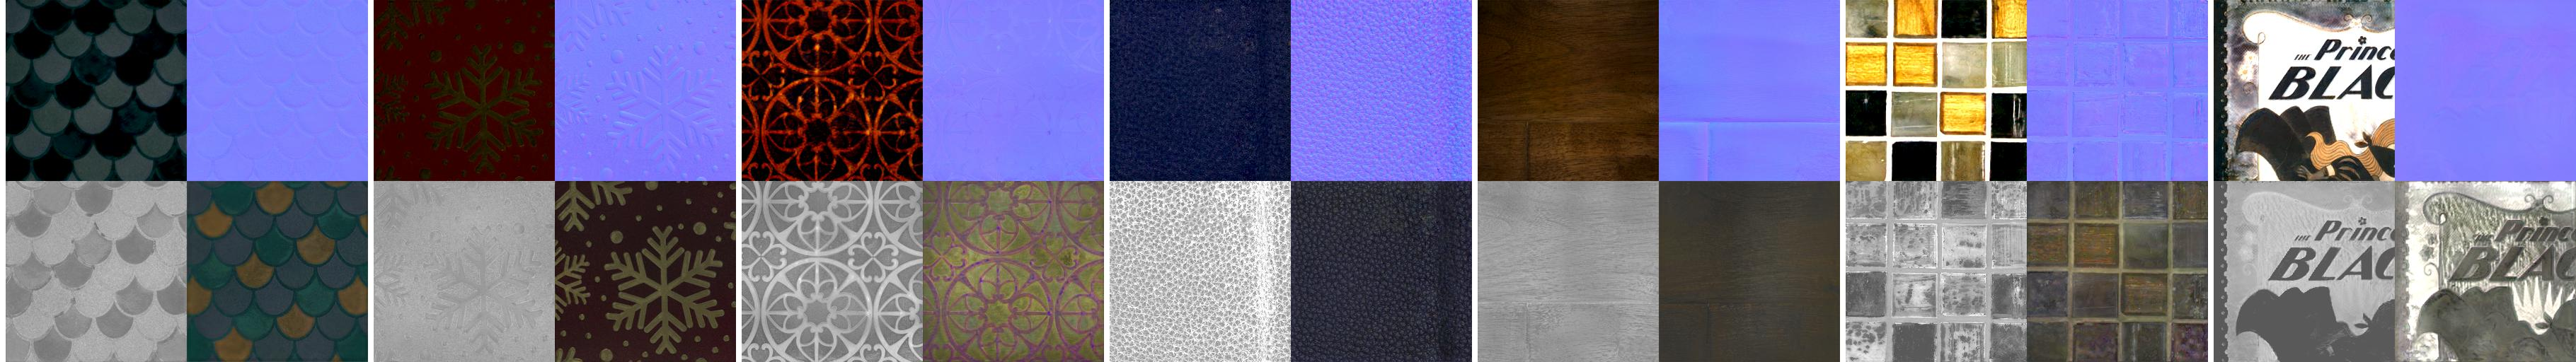
\includegraphics[width=\resLen]{teaser/maps.jpg}
	\end{tabular}
	\caption{\label{fig:teaser}
		We introduce a method to capture SVBRDF material maps from a small number of mobile flash photographs, achieving high quality results both on original and novel views. Our key innovation is optimization in the latent space of MaterialGAN, a generative model trained to produce plausible material maps; MaterialGAN thus serves as a powerful implicit prior for result realism. Here we show re-rendered views for several different materials under environment illumination. We use 7 inputs for these results (with 2 of them shown).
		(\textcolor{blue}{Please use Adobe Acrobat and click the renderings to see them animated.})
	}
\end{teaserfigure}
